\documentclass[10pt]{article}
\usepackage[letterpaper, margin=1in]{geometry}
\usepackage[utf8]{inputenc}
\usepackage[toc,page]{appendix}
\usepackage{amsmath, amsthm, amssymb, amsrefs}
\usepackage{graphicx}
\DeclareGraphicsExtensions{.pdf,.png,.jpg}
\usepackage{breqn}
\usepackage{alltt}
\renewcommand{\baselinestretch}{1.5}


%opening
\title{Tools and Ideas for the Proceedural Generation of Shadow Sculptures.}
\author{James Hoctor, Chris Chappell}

\begin{document}

\maketitle


\begin{abstract}
This paper discusses the creation of three dimensional objects,
given a shadow, a light source, and a wall, such that the object
creates the shadow on the wall when placed under the light source.
This problem was inspired by the artwork of Larry Kagan, a retired
professor at RPI. The use of genetic
algorithms to create these objects is discussed. A visualization
tool is described that shows how the object would look as a finished
product. We describe our respresentation of an object which is based
on the techniques Kagan uses in his art. An efficient way to
calculate the shadow cast by an object with this representation is
required in order to evaluate fitness in the genetic algorithm. We
describe our approach to shadow rendering. One component of fitness
in the genetic algorithm is the fidelity of the cast shadow to the
desired result. We discuss how we evaluate this degree of similarity.
Having described the means to evaluate the fitness of a
candidate object, we proceed to explain the recombination techniques
we suggest using to create each generation of objects from the parent generation.
\end{abstract}

\section*{Introduction}
This paper addresses the proceedural generation of artwork, if such
a thing is even possible. We wish to create art in the style of
Larry Kagan, whose medium is metal and the shadows it casts. In a
typical Kagan piece there is a metal object made from steel bars
that have been bent to shape and welded together to form a whole.
This assembly is mounted on a wall (painted white) and a spot light
shines on it to cast a shadow on the wall that forms an image. In a
naive sense, the problem  of creating something like Kagan's work is
a very simple one: one solution is to create a metal object in the shape of the desired
shadow but scaled down by half, then mount this half way between the
light source and the wall. The mounting can be done by means of
straight bars that travel in the shadow from the rest of the object
to the wall. But this is not the kind of result we desire. A major
challenge of this project is determining the other factors that make
a Kagan piece interesting beyond the mechanical fact that an image
is present in the form of a shadow. In particular, the metal portion
of a genuine Kagan is often visually chaotic and does not contain
recognizable forms. (Exceptions to this are discussed in the section
\ref{kagan}.) Our approach to generating artwork in this style
is therefore to use a genetic algorithm to search for a configuration
of metal that meets a variety of conditions among which is the
obvious requirement that the shadow appear as desired.

Other components of fitness of the object in the genetic algorithm
are its structural stability, its visual chaoticness, and its ability
to be fabricated using techniques similar to what Kagan uses. Structural stability
is addressed in section \ref{GA}. Visual
chaos is achieved by the random nature of the selection process.
Fabricability is included because it adds another constraint in a
problem that has few. It was key consideration when we decided
how to represent these sculptures.

\section{Larry Kagan's Work} \label{kagan}
In researching this problem we made a brief study of Kagan's work for
several reasons. Firstly, we wanted to identify a subset of his work
that might be most easily imitated. Secondly, our analysis shows how
necessary this restriction is. Kagan's work is too varied for the
whole body of work to be imitated. There is also the question of how
Kagan selects the image he wishes to create from shadow. In all of our
work we leave this crucial piece of creative heavy lifting to the
experts: humans.

Each of Larry Kagan's sculptures consists of a metal structure
composed of bent rods of metal mounted to a wall and illuminated by
a bright light from a carefully chosen location. The eye is drawn to
the shadow produced this way, which forms a familiar image, while the
rods themselves often have no obvious pattern. In the simplest case,
the shadow image is a line drawing and the rods are attached to the
wall at several points. For example, the piece ``Frankfurt Chair'' is
like this. Kagan has created many variations on this idea including
incorporating some of the bent rods in the recognizable image while
most of the image is formed by the shadow, as seen in ``Beach Chair''.
``Intersection of Two Circles'' shows that a sculpture composed of rods
can have a solid shadow with a geometric shape. The light source can
be on the ceiling cented over the piece or be off to one side as it
is in ``At''. With the light source on one side the shadow falls
predominantly on the side of the sculpture. Despite the fact that a
single small bright light source is installed to cast the shadow for
each sculpture, soft egdes of the shadow are noticeable in many of
these works. In ``Mosquito I'', Kagan uses this effect in a dramatic
way; the image present in the shadow of this sculpture is a mosquito
with its own shadow cast by an imaginary light source. In order to
make the distinction obvious, Kagan allowed soft shadow edges to show
in the portion of the image corresponding to the imaginary shadow of
the mosquito, but created the image of the mosquito with dark
hard-edged shadows. All of these sculptures (with the exception of ``At'') can be viewed on Larry Kagan's website \cite{Kagan}.

\section{How We Represent Sculptures and Why}
There are two different representations of sculptures used in this project. Both were chosen to make it likely that a sculpure that can be represented in our programs will be possible to make using techniques similar to Kagan's.

The first representation is used when saving a sculpure as a digital file. These files can be given as input to the visualization system that is described in section \ref{sculpture_render}. The informal specification of this format can be found in the file `ad file spec.txt' in the git repository submitted with this paper \cite{gitrepo}. An example file in this format can be generated by the script make-art-description.py, which is also in the git repository.

The contents of such a file include three things that represent the sculpture: the position of the light source (actually a list of point sources, so we can simulate a diffuse source), the radius of the bar stock to use in constructing the sculpture and a list of `strands'. Each strand is a list of points in 3D space, and it represents a space-filling shape composed of the union of spheres centered at each point and of cylinders with the centers of their end faces at consecutive points in the strand. The idea is that a strand approximates a smoothly bending piece of steel bar. One could construct the sculpture by making each strand from bar stock, then holding each strand in place and welding them together wherever they make contact.

This representation lends itself to checking whether the sculpture can be feasibly made or not. If any single strand cannot be made then the whole cannot. A strand might be impossible to make because it bends too sharply, or self intersects. The whole assembly might also fail to be fabricable if two strands intersect more than the small amount of intersection that would result from a weld. For comparison, one example of a representation that cannot be so easily checked for fabricability is a mesh of points describing the surface of the sculpture. This representation does lend itself to calculating shadows however.

The second representation that we use also makes use of the idea of spheres connected by cylinders. In fact, the representation is a simple graph with nodes representing the centers of spheres and edges representing cylinders connecting the centers of two spheres. This is the representation we propose using for the genetic algorithm.

Since any sculpture having a representation of the first kind has a representation of this second kind, but not vice versa, it is more likely that a sculpture with a representation of this second type will fail to be fabricable. Because of this, we propose that this representation be used with several checks. For example, one might check that no node has an order greater than 4 or 5, and that at least a certain percent of nodes have an order of 2 or fewer.

\section{How We Render Sculptures} \label{sculpture_render}
Using the method of spheres and cylinders, objects can be graphically modeled and displayed in 3D rendering systems fairly easily.  One method of doing this that we tested was using OpenGL to build a little engine that could render the object and a small surface such that the object and the shadow could be viewed from multiple angles, as it would look if it were printed.  The shadow could be imported as a texture, using OpenGL's \texttt{GL\_TEXTURE2D} object, and then fitted to the surface that would compose the wall.  This would allow modularity and would separate the methods that composed the creation of the shadow and its rendering.  While this may not be optimal, it is the most easily supported method using OpenGL legacy code.

\begin{figure}[h]
    \centering
    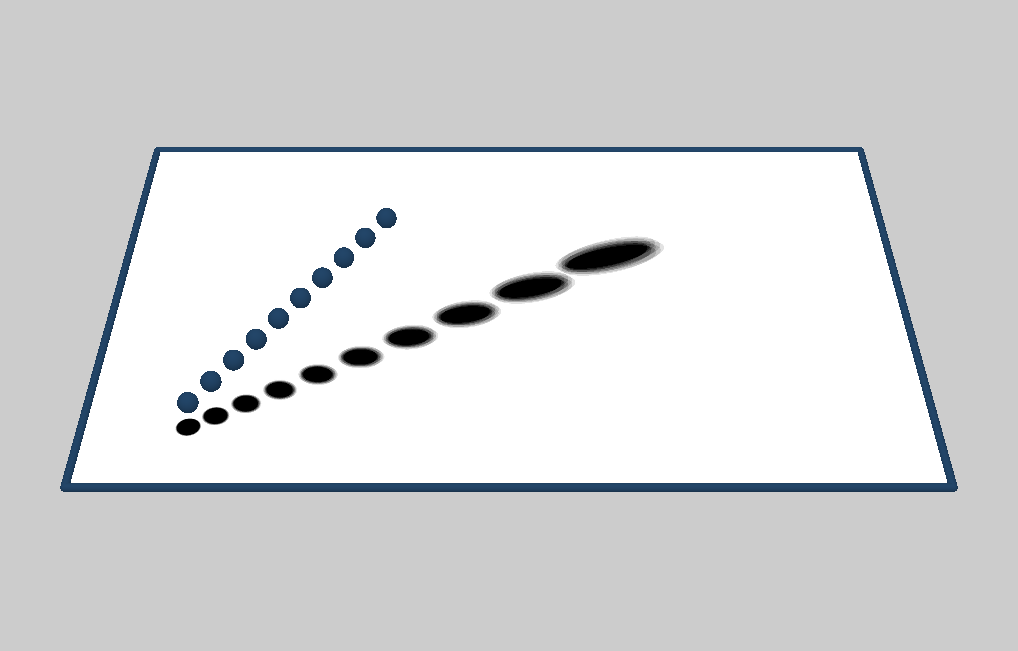
\includegraphics[width=0.8\textwidth]{object-render3.png}
    \caption{A sample render of ten spheres and their shadows.  The light source used was made up of nine point light sources, grouped together very closely.}
    \label{fig:render_3}
\end{figure}

To further explain the algorithm behind this method, first let us describe how the object would be represented.  The method used is most similar to the second representation of objects discussed previously, as spheres and cylinders in a graph layout.  Each object would consist of a list of nodes or spheres $W$, a list of edges or cylinders $E$, and a radius $r$.  The nodes in $W$ are described using 3-tuples of floating point numbers, representing their location in Cartesian 3-space, and the edges in $E$ are represented by 2-tuples of indexes, referencing the two nodes in $W$.  The algorithm iterates over the nodes in $W$, creating spheres of radius $r$.  Then, it iterates over the edges in $E$, and for each edge $e$ creates cylinders with radius $r$ and endpoints centered on the two nodes in $W$ indexed by $e$.  This is done using pyOpenGL's \texttt{gluSphere()} to draw spheres and \texttt{gluCylinder()} to draw cylinders.  For more information on the programming in this implementation, see \texttt{renderObject.py}.\cite{gitrepo}

For a more updated model that could possibly fix both the issue of slow shadow rendering time and separation of the shadow rendering from the object's rendering, one may instead of legacy OpenGL use OpenGL 3.3 or above, which adds the use of fragment shaders, and can render shadows from point light sources fairly easily.  The question that arises in this method, however, is how one would compare two shadows to determine accuracy and fitness of an object.  This would require further research and testing.

There are many video game engines that have builtin methods for shadow generation, with many options and customizable settings for doing so.  This may be the simplest option for rendering objects, and possibly even would also allow for comparison and heuristic generation.  Such engines would include Unity, Unreal Engine, and Source 2, just to name a few.  As our knowledge did not extend to the realm of writing video games, we felt more comfortable working with OpenGL.

\section{How We Render Shadows}
We investigated two CPU based ways to render the shadows of objects with a representation of the first kind (a list of strands). We believe that the increased speed of a GPU-based approach would be beneficial to the implementation of a genetic algorithm.

The first method is partially implemented in the file `rayTracing.py' on the branch `master' in the submitted git repository. In this method the cast shadow of each sphere and cylinder is computed individually and merged. Here is some pseudo-code for rendering the shadow of a collection of spheres and cylinders illuminated by a single point light source:

\begin{alltt}
input: \(\vec{l}\) = position of light
       \(r\) = the radius of each sphere and cylinder
       \(spheres\) = a list of positions of centers of spheres
       \(cylinders\) = a list of pairs of positions specifying the end faces of the cylinders
output: \(pixels\) = array of black and white pixels indicating on which areas of the wall
              light is incident

initialize \(pixels\) to be uniformly white (illuminated)

for each \(sphere\) in \(spheres\):
  if the sphere is entirely above the light or below the shadow plane:
    it casts no shadow; continue to the next sphere
  if the top of the sphere is beneath the light and the bottom is above the plane:
    The shadow cast on the plane will be elliptical.
    Calculate the equation of the cone formed by all lines passing through the
        light source and tangent to the sphere.
    Find the equation of the ellipse by intersecting this cone with the shadow
        plane.
    The equation has the form \(A*x^2 + B*y^2 + C*x*y + D*x + E*y + F = 0\).
    Rearrange the equation to have the form \(G(x)*y^2 + H(x)*y + I(x) = 0\), where
        \(G\), \(H\), and \(I\) are 2nd order or lower polynomials in x.
    For each column \(c\) in pixels:
      Find the value of \(x\) that corresponds to \(c\).
      Calculate \(G(x)\), \(H(x)\), and \(I(x)\).
      Use the quadratic formula to find two values of \(y\) satisfying the
          equation for the boundary of the ellipse.
      Convert the values of \(y\) to row coordinates in the image.
      In column \(c\) and all rows \(r\) between the two calculated:
        color \(pixels[r][c]\) black
  if the sphere intersects the shadow plane:
    Handling this case is at least as complicated as handling a sphere strictly
        above the plane.
    The circular intersection of the circle and the plane is shadowed.
    Any additional shadowing is a subset of the elliptical shadow described in
        the previous case.
    This case is not handled by our code.
  if the sphere intersects the light:
    Color all of pixels black.
    Return from the proceedure early.
    This case is not handled by our code.
  if the top of the sphere is above the light, its bottom below the light, without
      intersecting it:
    The shadow cast is hyperbolic.
    This case is not handled by our code, but it would likely be similar to
        the case of elliptical shadows.

for each cylinder in cylinders:
  //similar to the above but cylinders cast different shaped shadows
  // ...
  This case is not handled by our code.
\end{alltt}

This proceedure needs to be repeated for each point light source, creating a separate image for each. Then these images need to be averaged, pixel by pixel. When generating a 1024x720 image of the shadow this averaging process took about 1.2 seconds for our python implementation. With a 3000x3000 image it took almost 13 seconds. It should be possible to take advantage of data parallelism here and do the averaging process in OpenGL on a GPU, or perhaps with single instruction multiple data technologies like SSE and AVX.

We did not implement casting the shadows of cylinders by this method, but there is an optimization that deserves mention. It results from the fact that we can assume there is a sphere present at each end of any cylinder. Consequentially, any cylinder that is aligned with one face toward the light source casts a shadow only where a sphere has already cast a shadow. The optimization that arises from this is to ignore cylinders with such an orientation in the loop over all cylinders.

Furthermore, even when the cylinder is not aligned this way we can skip drawing the portion of the shadow that results from the end faces, for the same reason. In this case, the shadow drawn for a cylinder would be a quadrilateral. Imagine two planes, each of which is tangent to the circular wall of the cylinder and passes through the point light source. They are tangent on opposite sides of the cylinder. Each plane has an intersection point with each circular face of the cylinder. The four such intersection points are co-planer, and the quadrilateral they form is entirely inside the cylinder. The shadow of this quadrilateral is thus a part of the shadow of the cylinder. The remaining part of the cylinder's shadow should also be shadowed by the spheres.

Appendix \ref{a} presents a derivation of the equation of the elliptical boundary of the shadow of a sphere in the most typical case.

In an attempt to render shadows more quickly, another technique was attempted. The code for this technique can be found in the newRayTracing branch of the git repository. This second method is a refinement of the following naive method:

Suppose you have a pair of proceedures that are used to efficiently check whether a line segment intersects a sphere or a cylinder. You can iterate over the lights, and over all the pixels in the image, and construct the line segment from the light to the center of the pixel. Then go through all the spheres and cylinders checking for an intersection. At the first intersection, the light intensity at the pixel is decremented and we move on to the next pair of a light and a pixel. The motivation behind this method is that there is no step of merging the shadow of each point light source. [Consider writing out pseudo code for this.]

The innermost loop (over all spheres and cylinders) can be accelerated by use of a space partitioning method.

The refinement that can be added is simplest to understand if we restrict ourselves temporarily to intersections with spheres. For each light source we imagine a pyramid with the region-of-interest of the shadow plane as its base and the light source as its vertex. We divide the pyramid into chunks and to each chunk associate all the spheres with a center near the chunk. When checking if a line segment inersects any sphere, we can ignore any sphere not in a chunk near the line segment. OK, but how do we organize this in practice? In our implementation, the pyramid is first divided into horizontal regions...

[Mention inspiration from nearest neighbor algorithm]


It should also be very fast to render shadows using openGL. Shadowmaps are a standard technique for rendering dynamic shadows. In shadowmapping, a scene is rendered from the perspective of a point light source and the resulting ``image'' is colored according to how far each part of the image is from the light. Shadowmapping typically goes on to use this information to shade a rendering of the same scene from another perspective, but we only want an image of the shadow on the wall.

\section{Genetic Algorithm Solutions} \label{GA}
We believe approximate solutions to the forward problem may be possible using genetic algorithms for creating ``abstract'' data that fits a given shadow.  The question then becomes how to represent data for each possible solution to the problem in a genome that allows simple crossovers and mutations.  Some possible representations are as follows: 

The simplest method of representing nodes and edges would be to keep the number of both constant, moving the nodes around while retaining the same edge mappings for all genomes.  This way, one could represent each node as an unsigned integer, or an array of three unsigned integers representing the positive incremental distance from some origin point.  Given the nature of the problem, one can disregard any space not within the projection from the light source to a given section of the wall.  This allows the bounding of the entire system in a cube, which we can use to define our \texttt{0} and our \texttt{MAX\_INT} for each coordinate direction.  Next, we would create an array of unsigned integers, of length 3 times the number of nodes in the system.  This would be the genome for the genetic algorithm.  The fitness function would be defined as the number of matching pixels (within a certain threshold) between the input and the generated shadow using one of the shadowmapping methods above.  Using such a method would prevent situations where the graph became unconnected, but it does not address issues of structural integrity any further than this.  Since the nature of the problem allows for many local solutions, the ability of such a genetic algorithm to converge may be slowed.

One may increase the variability of the genetic algorithm by introducing edge mapping to the genome.  One may represent an edge between node A and node B as a 1 in a symmetric n-by-n adjacency matrix, where n is the number of nodes in the graph.  This allows for easy genetic recombinations, with the ability to vary the number of edges in the graph.  The issue that this does not take care of is the connectivity of the graph.  One would have to either add a penalty to the fitness function which performed a depth-first search on the nodes and penalized unconnected graphs, or alternatively, one could modify the base constructs of the genetic algorithm, making it continue to perform attempts at combining two genomes until it had children that were all fully connected.  For the first option, the question would become how strongly one would decrease the fitness of an unconnected graph, and whether the number of unconnected pieces should increase that penalty.  The second option would allow us to use the same fitness function, but may add extra levels of complexity to the problem due to the required repeated attemps within single generations.

The last important part of the genetic algorithm is a method of performing mutations on genomic data.  Here are some options in consideration:

By simply mutating the data in the genome, one would cause one or multiple nodes to be moved to a new location, possibly on the same plane, but possibly not.  This would be the simplest method of performing a mutation, but depending on how the nodes are laid out, it may mutate a node outside of the acceptable region given for nodes in the given problem.  Whether this is allowed or not depends on the situational requirements given.

Another mutation would be to swap the position of two nodes.  This would not require any checking to see whether any node is outside the mapped region, but it would not add anything new to the domain of a generation from the previous generation, unless there was little or no variation of edges in the whole generation.

Mutations can also be performed on edge data.  This can simply be done by inverting bits in the adjacency matrix, which would cause edges to disappear or new edges to occur.  This could be used along with the first mutation option to give the complete range of options for convergence, barring adding or removing nodes themselves.  The downside to this form of mutation is that it could make the graph unconnected, which, like doing combinations on edges, would require either some penalty in the fitness function, or a checker to make sure any edge that is removed is not required to keep the graph fully connected.

\section{Future Work}
What is the best way to use point sources to simulate a diffuse light source? Is there a better way than point light sources to simulate a diffuse source?

How can the partitioning of space in the second rendering method be improved to allow faster shadow drawing? More equally sized partitions? Adaptively sized partitions?

The inverse square law is not respected by our shadow drawing algorithms. (Does this Include the OpenGL one?) Can this law be incorporated into our algorithms? Is it even necessary to include this or does the human visual system ignore this variation in brightness? Mention the image processing technique histogram equalization.

The visualization tool lacks the ability to draw shadows cast on the object by itself. These shadows are not an important component of Kagan's art as far as we can tell.

Is it a good idea to combine the two cpu-based shadow-rendering techniques? For example, use the second method to draw spheres and the first to draw cylinders?

We should use bresenham's algorithm to draw an ellipse once we have its parameters, instead of the naive method we use now.

\begin{appendices}
\chapter{A} \label{a}

In this appendix we will show in detail the calculation of the boundary of a shadow cast by a sphere by a point light source. The shadow is cast on the $z=0$ plane. On the z-axis the sphere is strictly between the light and the plane. We are given $\vec{l}$, the location of the point light source, $\vec{c}$, the center of the sphere, and $r$, its radius.

The first step is to derive the equation of the shadow cone. A generic point on the cone will be denoted by $\vec{s}$. The axis of the cone passes through $\vec{l}$ and through $\vec{c}$. The defining property of $\vec{s}$ is 
\begin{equation}\label{sproperty}
\|orth_{\vec{c}-\vec{l}} (\vec{s} - \vec{l})\| = \|proj_{\vec{c}-\vec{l}} (\vec{s} - \vec{l})\| \cdot k
\end{equation}
where $k$ is a constant characteristic of the aperture of the cone. Equation (\ref{sproperty}) says that the distance of a point from the cone's axis is in constant proportion to its distance along the axis. The value of $k$ can be calculated from any point on the cone. We will calculate $k$ from the projection and orthogonal projection of a point of tangency, $\vec{p}$, of the sphere and cone.

The vector $\vec{p} - \vec{l}$ is along a generatrix of the cone, so it is perpendicular to $\vec{p} - \vec{c}$, which points from the center of the sphere to the point of tangency (see figure \ref{fig:shadow_1}). Therefore, a right triangle is formed by $\vec{p}$, $\vec{c}$, and $\vec{l}$, with $\vec{c}$ and $\vec{l}$ at the ends of the hypotenuse. The length $L=\|\vec{c}-\vec{l}\|$ can be calculated from the givens and the distance $r=\|\vec{p}-\vec{c}\|$ is a given. By the pythagorean theorem the length of the other leg is $L'=\|\vec{p}-\vec{l}\|=\sqrt{L^2-r^2}$. In figure \ref{fig:shadow_2} the triangle formed by the projection and orthogonal projection of $\vec{p}-\vec{l}$ onto $\vec{c}-\vec{l}$ is shown with the triangle formed by $\vec{p}$, $\vec{c}$, and $\vec{l}$. The triangles are similar because they share two congruent angles. Thus their sides have the same proportions. In particular:
\[
k = \frac{\|orth_{\vec{c}-\vec{l}} (\vec{p} - \vec{l})\|}{\|proj_{\vec{c}-\vec{l}} (\vec{p} - \vec{l})\|} = \frac{r'}{L''} = \frac{r}{L'} = \frac{r}{\sqrt{L^2-r^2}}
\]

\begin{figure}[ht]
    \centering
    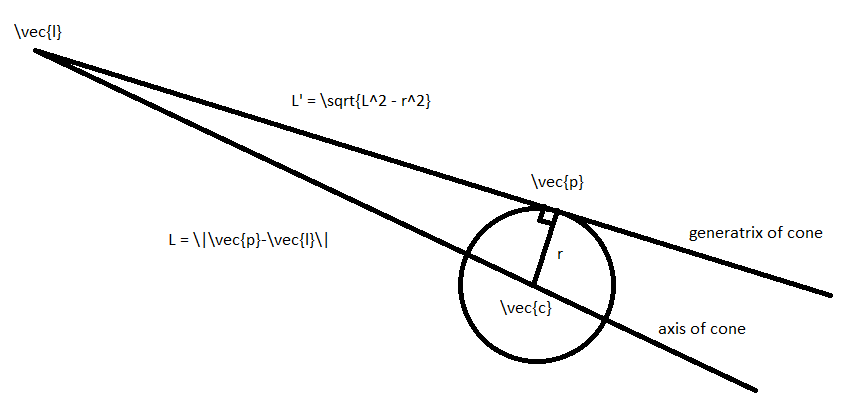
\includegraphics[width=0.8\textwidth]{sphere_shadow_figure_1.png}
    \caption{Depicted is the light source, a sphere, and a ray of light tangent to the sphere (labeled as generatrix of cone).}
    \label{fig:shadow_1}
\end{figure}

\begin{figure}[ht]
    \centering
    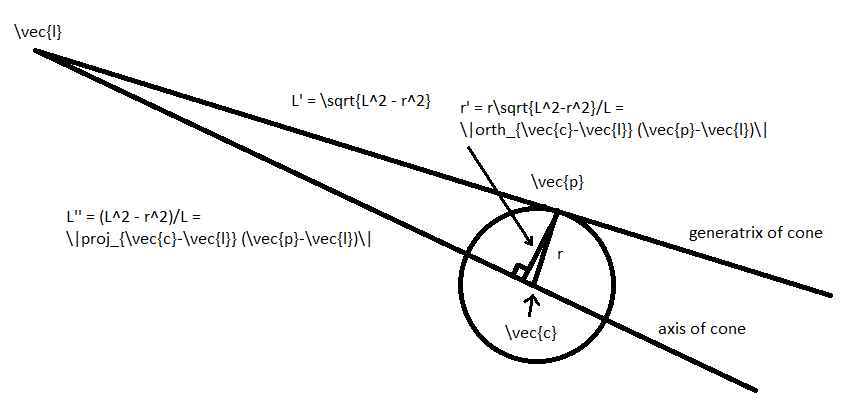
\includegraphics[width=0.8\textwidth]{sphere_shadow_figure_2.png}
    \caption{This figure includes in addition the orthogonal projection from the point of tangency to the axis of the cone. The distance $L''$ is from the light source to the tip of the projection vector.}
    \label{fig:shadow_2}
\end{figure}

%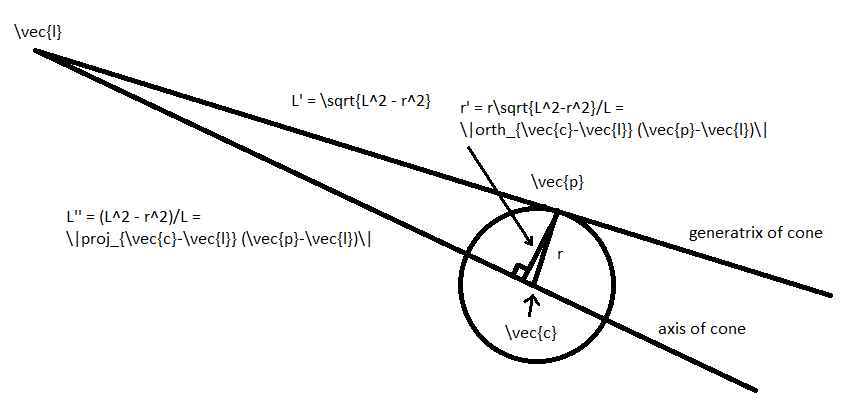
\includegraphics[scale=0.60]{sphere_shadow_figure_2}

Now we use the defintions of $orth_{\vec{u}} \vec{v}$ and $proj_{\vec{u}} \vec{v}$ to simplify equation (\ref{sproperty}).
\begin{align*}
proj_{\vec{u}} \vec{v} &= \vec{u} \frac{\vec{u}\cdot\vec{v}}{\vec{u}\cdot\vec{u}}\\
orth_{\vec{u}} \vec{v} &= \vec{v} - proj_{\vec{u}} \vec{v}
\end{align*}
Start by squaring both sides of \ref{sproperty} and substituting. Let $\vec{d} = \vec{c}-\vec{l}$, $\vec{t} = \vec{s}-\vec{l}$.
\begin{align*}
\|\vec{t} - \vec{d} \frac{\vec{d}\cdot\vec{t}}{\vec{d}\cdot\vec{d}}\|^2 &= \|\vec{d} \frac{\vec{d}\cdot\vec{t}}{\vec{d}\cdot\vec{d}}\|^2 \cdot k^2\\
\vec{t}\cdot\vec{t}-2\vec{t}\cdot\vec{d} \frac{\vec{d}\cdot\vec{t}}{\vec{d}\cdot\vec{d}}+\vec{d}\cdot\vec{d}(\frac{\vec{d}\cdot\vec{t}}{\vec{d}\cdot\vec{d}})^2 &= (\vec{d}\cdot\vec{d}) (\frac{\vec{d}\cdot\vec{t}}{\vec{d}\cdot\vec{d}})^2 \cdot k^2
\end{align*}
Multiply each side by $\vec{d}\cdot\vec{d}$:
\begin{align*}
(\vec{t}\cdot\vec{t})(\vec{d}\cdot\vec{d})-2(\vec{d}\cdot\vec{t})^2+(\vec{d}\cdot\vec{t})^2  &= (\vec{d}\cdot\vec{t})^2 \cdot k^2\\
(\vec{t}\cdot\vec{t})(\vec{d}\cdot\vec{d})-(\vec{d}\cdot\vec{t})^2 & = (\vec{d}\cdot\vec{t})^2 \cdot k^2
\end{align*}
Divide both sides by $k^2$ and substitute $k^2 = r^2 / ( L^2-r^2)$.
\begin{align*}
((\vec{t}\cdot\vec{t})(\vec{d}\cdot\vec{d})-(\vec{d}\cdot\vec{t})^2)\cdot ( L^2-r^2)/r^2 &=  (\vec{d}\cdot\vec{t})^2\\
(\vec{t}\cdot\vec{t})(\vec{d}\cdot\vec{d})( L^2-r^2)/r^2 &=  (\vec{d}\cdot\vec{t})^2(1 + ( L^2-r^2)/r^2)\\
(\vec{t}\cdot\vec{t})(\vec{d}\cdot\vec{d})( L^2-r^2)/r^2 &=  (\vec{d}\cdot\vec{t})^2 L^2/r^2
\end{align*}
The quantities $\vec{d}\cdot\vec{d}$ and $L^2$ are equal (see figure \ref{fig:shadow_1}).
\begin{equation}\label{coneeqn}
(\vec{t}\cdot\vec{t})( L^2-r^2) =  (\vec{d}\cdot\vec{t})^2
\end{equation}
Now we find the intersection of this cone with the $z=0$ plane. Let $x$ and $y$ be coordinates on the shadow plane. The condition for intersection is that the third component of $\vec{s}$ be $0$. We put $\vec{t}$ and $\vec{d}$ in terms of $x$ and $y$ and substitute into equation \ref{coneeqn}.
\begin{align*}
\vec{s}& = \langle x,y,0 \rangle\\
\vec{d}\cdot\vec{t} &= \vec{d}\cdot\vec{s} - \vec{d}\cdot\vec{l} = d_1x+d_2y - \vec{d}\cdot\vec{l}\\
\vec{t}\cdot\vec{t} &= \vec{s}\cdot\vec{s} -2\vec{s}\cdot\vec{l} + \vec{l}\cdot\vec{l} = x^2 + y^2-2l_1x-2l_2y+ \vec{l}\cdot\vec{l}\\
(\vec{d}\cdot\vec{t})^2 &= (d_1x+d_2y - \vec{d}\cdot\vec{l})^2\\
&= (d_1x+d_2y)^2 - 2(d_1x+d_2y)(\vec{d}\cdot\vec{l}) + (\vec{d}\cdot\vec{l})^2\\
&= d_1^2x^2+2d_1d_2xy+d_2^2y^2-2d_1x(\vec{d}\cdot\vec{l})-2d_2y(\vec{d}\cdot\vec{l})+(\vec{d}\cdot\vec{l})^2\\
&= d_2^2y^2 + (2d_1d_2x -2d_2(\vec{d}\cdot\vec{l}))y + (d_1^2x^2-2d_1x(\vec{d}\cdot\vec{l})+(\vec{d}\cdot\vec{l})^2)\\
(\vec{t}\cdot\vec{t})( L^2-r^2) &= (x^2 + y^2-2l_1x-2l_2y+ \vec{l}\cdot\vec{l})(L^2-r^2)\\
&= (L^2-r^2)y^2 + (-2l_2(L^2-r^2))y + (x^2-2l_1x+ \vec{l}\cdot\vec{l})(L^2-r^2)
\end{align*}
For the final result we subtract the one side of equation \ref{coneeqn} from the other to obtain:
\begin{dmath*}
0 = (\vec{d}\cdot\vec{t})^2 - (\vec{t}\cdot\vec{t})( L^2-r^2)\\
= (d_2^2 - (L^2-r^2))y^2 + (2d_1d_2x -2d_2(\vec{d}\cdot\vec{l})+2l_2(L^2-r^2))y+(d_1^2x^2-2d_1x(\vec{d}\cdot\vec{l})+(\vec{d}\cdot\vec{l})^2 - (x^2-2l_1x+ \vec{l}\cdot\vec{l})(L^2-r^2))
\end{dmath*}

\end{appendices}
% ftp://ftp.ams.org/ams/amsrefs/amsrdoc.pdf for amsrefs documentation
\begin{bibdiv}
 \begin{biblist}
  \bib{Dasgupta}{book}{
   title={Algorithms},
   author={Dasgupta, Sanjoy},
   author={Papadimitriou, Christos},
   author={Vazirani, Umesh},
   publisher={McGraw-Hill Education},
   address={New York},
   year={2006}  
  }
  \bib{pyOpenGL}{webpage}{
   title={PyOpenGL Documentation},
   url={http://pyopengl.sourceforge.net/documentation/},
   accessdate={2015-10}
  }
  \bib{gitrepo}{webpage}{
   title={Genetic Algorithms for Shadow Sculptures},
   author={Chris Chappell},
   author={James Hoctor},
   url={https://github.com/chappc/Math-Senior-Research},
   accessdate={2015-12}
  }
  \bib{cylindermagic}{webpage}{
   title={Rendering a Cylinder Between Two Points in OpenGL},
   author={Parris, Joel},
   url={http://lifeofaprogrammergeek.blogspot.com/2008/07/rendering-cylinder-between-two-points.html},
   accessdate={2015-10}
  }
  \bib{opengl-tutorial}{webpage}{
   title={opengl-tutorial},
   url={http://www.opengl-tutorial.org/},
   accessdate={November 2015}
  }
  \bib{Kagan}{webpage}{
   title={Larry Kagan Sculpture},
   url={http://larrykagansculpture.com/},
   accessdate={October 2015}
  }
 \end{biblist}
 
\end{bibdiv}


\end{document}
